\documentclass[letterpaper]{article}
\usepackage{amsmath}
\usepackage{array}
\usepackage{color}
\usepackage{graphicx}
\usepackage{float} % utiliser H pour forcer a mettre l'image ou on veut
\usepackage{lscape} % utilisation du mode paysage
\usepackage{mathbbol} % permet d'avoir le vrai symbol pour les reels grace a mathbb
\usepackage{enumerate} % permet d'utiliser enumerate
\usepackage{moreverb} % permet d'utiliser verbatimtab : conservation la tabulation
\usepackage{stmaryrd} % permet d'utiliser \llbrackedt et \rrbracket : double crochet
\usepackage[noabbrev]{cleveref} % permet d'utiliser cref and Cref
\usepackage{caption} % permet d'utiliser subcaption
\usepackage{subcaption} % permet d'utiliser subfigure, subtable, etc
\usepackage[margin=1.in]{geometry} % controle les marges du document
\usepackage{algorithm}
\usepackage{url}


\newcommand\bn{\boldsymbol{\nabla}}
\newcommand\bo{\boldsymbol{\Omega}}
\newcommand\br{\mathbf{r}}
\newcommand\la{\left\langle}
\newcommand\ra{\right\rangle}
\newcommand\bs{\boldsymbol}
\newcommand\red{\textcolor{red}}
\newcommand\ldb{\{\!\!\{}
\newcommand\rdb{\}\!\!\}}
\newcommand\llb{\llbracket}
\newcommand\rrb{\rrbracket}

\renewcommand{\(}{\left(}
\renewcommand{\)}{\right)}
\renewcommand{\[}{\left[}
\renewcommand{\]}{\right]}


\begin{document}
\title{Parallel $S_n$ Sweeps on Adapted Mesh}
\author{Bruno Turcksin} 
\date{}
\maketitle

\begin{abstract}
  TODO
\end{abstract}

% In the paper, they gave a weight of 1/3 instead of zero to the arcs between
% two different processors.
\section{Introduction}
When using the discrete ordinates method to discretize the transport equation,
it is usually necessary to sweep multiple times through the mesh. Sweeping in
parallel through a mesh can be viewed as a resource-constrained project
scheduling problem (RCPSP) \cite{Brucker1999,Kolisch2006}. RCPSP has been
extensively studied for more than four decades \cite{Pritsker1969} but most
sweeping algorithms have been developed independently of these researches. In
\cite{Adams2013}, a family of optimal sweeping algorithms is described for
regular grids. For unstructured grids, several heuristics have been proposed
over the years \cite{Pautz2002,Plimpton2005,Yan2013,Colomer2013,Kumar2005}. When
studying sweeping algorithms, it is necessary to also study the partitioning of
the mesh. Two identical meshes partitioned differently will lead to different
optimal scheduling. Therefore, to obtain the best speed up given a mesh and a
number of processors, the sweeping algorithm and the partitioning should be
studied together. However, in this paper, we will assume that the partitioning
is given. This is representative of the case where the partitioning is done by a
third-party library or when the partitioning cannot be tailored for the
transport equation because others physics must be accounted for. We will focus
our study on refined meshes
\cite{Arnold2000,Baker2002,Bangerth2007,Jessee1998,Wang2010a}. In this paper, we
study the CAP-PFB algorithm defined in \cite{Mo2014} which is based on a widely
used method in RCPSP introduced in \cite{Li1992}. In particular, we will study
how the algorithm behaves on regular grids and how it can modified for mesh
constructed using adaptive mesh refinement (AMR). This work will show some
preliminary results on the performance of sweeps on meshes similar to the ones
produced by deal.II \cite{Bangerth2007,Bangerth2013} and p4est
\cite{Burstedde2011}. Deal.II is an open source finite element library which
uses the p4est library for the partitioning. The rest of this paper is organized
as follows: in \Cref{parallel_sweeps}, we explain the CAP-PFB algorithm
introduced in \cite{Mo2014} and we show how to apply it to adapted mesh. In
\Cref{results}, we show some results, first on an uniform mesh where the optimal
solution is known and then, on meshes more typical of what is obtained using
AMR. We end with our conclusions in \Cref{conclusions}.


\section{Parallel sweeps on AMR mesh} \label{parallel_sweeps}
\subsection{CAP-PFB algorithm}
In this Section, we explain the CAP-PFB (Cut Arc Preference - Parallel Forward
Backward) algorithm introduced in \cite{Mo2014}. We will start with the general
Forward-Backward (FB) algorithm \cite{Li1992}. This algorithm has been developed
to schedule a set of tasks given dependencies between the tasks and constraints
on the resources. It is based on the observation that when we try to execute the
tasks as soon as possible, a lot of work is done at the beginning of the
schedule but it quickly decreases and there is only few tasks to perform later
on. The opposite is true when we try to execute the tasks as late as possible,
few tasks are performed at the beginning but a lot of them are done at the end
of the schedule. The idea of the FB iterations is to alternate a phase where the
tasks are executed as early as possible (forward iteration) with a phase where
the tasks are executed as late as possible (backward iteration). The hope is
that we will get a more constant distribution of the work and therefore,
decrease the time needed to execute all the tasks. The algorithm works as
follow:
\begin{algorithm}[H]
  \caption{FB algorithm}
  \begin{itemize}
    \item Start with an initial scheduling.
    \item Iterate until convergence or maximum number of steps:
      \begin{enumerate}
        \item Forward iteration:
          \begin{enumerate}
            \item Compute the ranks of the tasks.
            \item Sort the tasks in ascending order of the ranks.
          \end{enumerate}
        \item Backward iteration:
          \begin{enumerate}
            \item Compute the ranks of the tasks.
            \item Sort the tasks in descending order of the ranks.
          \end{enumerate}
      \end{enumerate}
  \end{itemize}
\end{algorithm}
PFB is the parallel version of FB. If the forward iteration is done after the
backward iteration, one
FB iteration will end with a forward sweep. Different FB
algorithms will differ by the method used to compute the ranks of the tasks. The
Cut Arc Preference (CAP) method uses a graph to represent the dependency of the
task. The cut arcs are the arcs between tasks (vertices of the
graph) owned by different processors. The ranks as computed as follows:
\begin{itemize}
  \item Backward iteration rank of a task: earliest start time of all its downstream tasks
    owned by a different processor. Tied are broken using the own task start time.
    %$\min_{(v_k,v_j)\in S_i}\left\{s_j-w_{k,j}\right\} \cup \left\{+\infty\right\}$
  \item Forward iteration rank of a task: latest end time of all its upstream tasks owned
    by a different processor. Tied are broken using the own task end time.
    %$\max_{(v_j,v_k)\in B_i} \left\{f_j+w_{j,k}\right\} \cup \left\{-\infty\right\}$
\end{itemize}
\subsection{CAP-PFB on adapted mesh}
In \Cref{subdomain_id}, we show the partitioning of mesh using deal.II and p4est 
on 16 processors. This is a typical mesh produced by these libraries and it is
representative of the case that we want to tackle. 
\begin{figure}[H]
  \begin{subfigure}[b]{.5\textwidth}
    \centering
    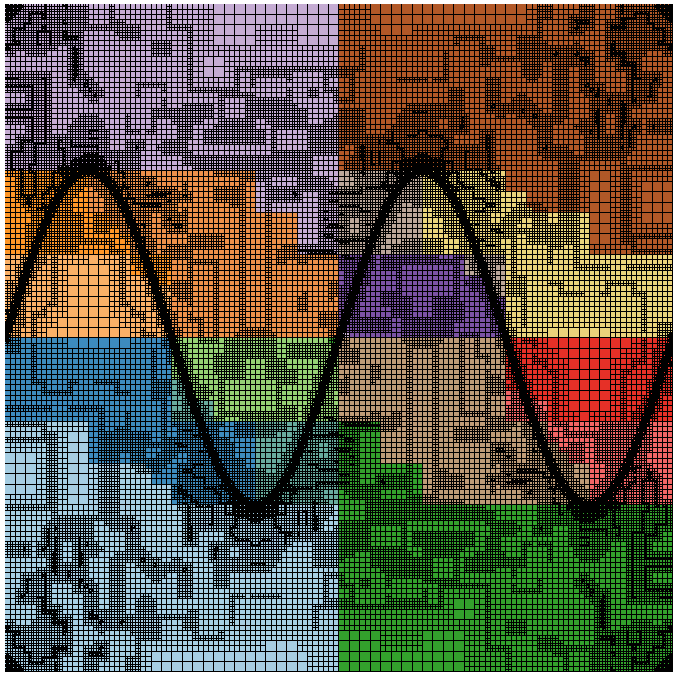
\includegraphics[width=5cm]{subdomain_id_0}
    \caption{Partitioning and mesh.}
  \end{subfigure}
  \begin{subfigure}[b]{.5\textwidth}
    \centering
    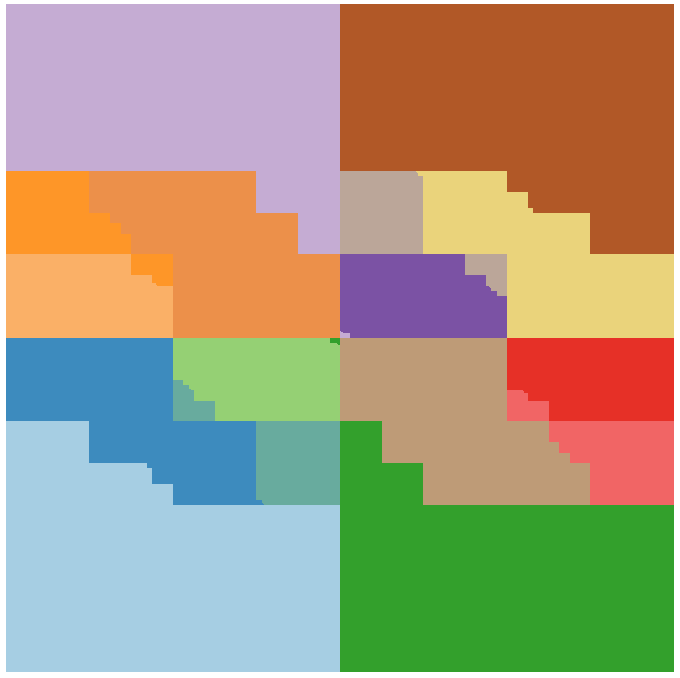
\includegraphics[width=5cm]{subdomain_id_1}
    \caption{Partitioning.}
  \end{subfigure}
  \caption{Partitioning and mesh using 16 processors for a typical problem
  (Step-40).}
  \label{subdomain_id}
\end{figure}
We can see that the domain owned by each processors are not convex and that some
processors own disjoint domains. In \cite{Mo2014}, the authors studied CAP-PFB
when all the tasks have an equal amount of work to execute. In this case,
CAP-PFB is guarantee to converge some scheduling. This can be achieved by using
tasks that are associated to only one cell. However, this will create an
excessive amount of messages which will negatively impact the performance
\cite{Pautz2002}. Therefore, it is necessary to have tasks that cover more than
one cells. On a totally unstructured mesh, gathering cells to form convex zones
can be a hard problem. However, this can be easily done on an AMR mesh since the
children of a coarse cell can be gather to form a convex zone, i.e. the parent
cell. It is of course necessary that all the children are owned by the same
processor. Otherwise, a task would span over multiple processors. This process
can be extended to grand-children, great-grand-children, etc. This will create
tasks that have very different numbers of cells associated to them either
because some cells have less ancestors or because some cells that have a common
ancestors are owned by different processors. Having tasks containing different
numbers of cells can be  taken into account in CAP-PFB but the resulting
algorithm loses its convergence property. We will show in \Cref{results} that
the number of stages of successive scheduling oscillates. Because the best
solution can be obtained after a poor one, it is hard to check for convergence.
To fix this undesirable behavior, scheduling that increase the number of stages
will be rejected and instead, the best scheduling will be used by the following
forward/backward iteration.


\section{Results} \label{results}
In this Section, we look at the number of stages produced by the CAP-PFB
heuristic. In the first test, we compared the sweep ordering produced by CAP-PFB
with the optimal solution on an uniform mesh. In the second and third tests, we
look at the ordering on AMR meshes. In all the tests, the domain is square and
we use a $S_8$ quadrature, i.e. 40 directions. When CAP-PFB is known to have an
oscillatory behavior, we will performed 20 CAP-PFB iterations. Otherwise, we
will stop when an iteration does not improve the scheduling.
\subsection{Uniform mesh}
In this test, we compare the number of stages on an uniform two-dimensional mesh 
where each processors owns 40 tasks (one task for each direction). In this
setup, the optimal number of stages is given by \cite{Adams2013}:
\begin{equation}
  \mu = P_x + P_y - 4 + N_{\textrm{task}},
\end{equation}
with $P_x \times P_y$ the process grid and $N_{\textrm{task}}$ the number of
tasks that each processors has to executed. Because CAP-PFB
is an heuristic that requires an initial scheduling, we use three different
initial scheduling for each test. In \Cref{uniform}, we compare the number of
stages obtained using CAP-PFB to the optimal solution for different meshes.
% Order of results: no seed, seed = 0, seed = 1.
% TODO: if enough time do 70 \times 70 it should be much faster now
\begin{table}[H]
  \begin{center}
    \begin{tabular}{|c|c|c|c|c|}
      \hline
      N. procs & Init. n. stages & Final n. stages & Optimal n. stages & Iter. \\
      \hline
      $10\times 10$ &  580 &  56 &  56 & 1 \\
      $10\times 10$ &  155 &  56 &  56 & 2 \\
      $10\times 10$ &  153 &  56 &  56 & 1 \\
      $30\times 30$ & 1780 &  96 &  96 & 1 \\
      $30\times 30$ &  392 &  96 &  96 & 2 \\
      $30\times 30$ &  376 &  96 &  96 & 2 \\
      $50\times 50$ & 2980 & 136 & 136 & 1 \\
      $50\times 50$ &  570 & 136 & 136 & 2 \\ 
      $50\times 50$ &  573 & 136 & 136 & 2 \\
      \hline
    \end{tabular}
    \caption{Number of stages required to sweep through an uniform mesh.
      \emph{N. procs} is the number of processors, \emph{Init. n. stages} is the
      number of stages of the initial scheduling, \emph{Final n. stages} is the
      number of stages of the final scheduling, \emph{Optimal n. stages} is the
      number of stages of the optimal scheduling, and \emph{Iter.} is the number
    of CAP-FBS performed.}
    \label{uniform}
  \end{center}
\end{table}
We can see that the heuristic converges to the optimal solution in only one or
two iterations for every initial scheduling. Even if the number of stages is
identical, the final scheduling obtained using different initial scheduling are
different.

\subsection{First AMR test}
In this test, the cells in the middle of the domain are refined (\Cref{mesh_1}).
The red squares represent the processors and the black squares represent cells
or sets of cells. Forty tasks, each one requiring one unit of work, are
associated to each black square.
\begin{figure}[H]
  \centering
  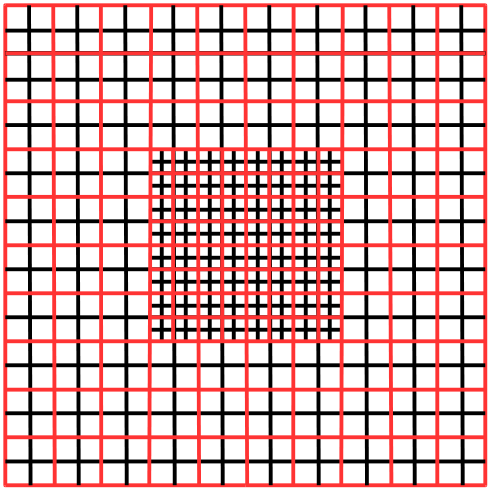
\includegraphics[width=5cm]{mesh}
  \caption{Mesh refined in the middle of the domain.}
  \label{mesh_1}
\end{figure}
First, we test the case where each processors owns 160 tasks (\Cref{amr_1}).
% Order of results: no seed, seed = 0, seed = 1.
% Table for amr_0 = refined mesh in the middle have NOT been gather
\begin{table}[H]
  \begin{center}
    \begin{tabular}{|c|c|c|c|}
      \hline
      N.procs & Init. n. stages & Final n. stages & Iter. \\
      \hline
      148 & 1870 & 238 & 2 \\
      148 &  911 & 247 & 3 \\
      148 &  923 & 246 & 3 \\
      592 & 3820 & 332 & 3 \\
      592 & 1552 & 336 & 6 \\
      592 & 1598 & 341 & 4 \\
      \hline
    \end{tabular}
    \caption{Number of stages required to sweep through a mesh refined
    in the middle of the domain.}
    \label{amr_1}
  \end{center}
\end{table}
We can see that different initial sweeps produce sweeps requiring different
number of stages. The best results are obtained when the initial sweep goes
through the mesh along one direction at the time. In the others cases, the sweep
can stall at the beginning because instead of pushing the front wave forward and
allowing other processors to start working, tasks on the corners of the domain
are executed first. This slows downs the front wave. The sensitivity of the
algorithm to the initial sweep is due to the fact that the order of tasks that
have the same ranks cannot be changed. This allows to make sure the precedence
relationships are always satisfied without having to check them. 

Next, the tasks in the refined area are gathered together. Therefore, the
processors of this zone do not own 160 tasks, each requiring one unit of work to
be executed, but 40 tasks, each requiring four units of work to be executed
(\Cref{amr_2}). 
% Order of results: no seed, seed = 0, seed = 1.
% Table for amr_1 and amr_3 = refined mesh in the middle have been gather
\begin{table}[H]
  \begin{center}
    \begin{tabular}{|c|c|c|c|}
      \hline
      N.procs & Init. n. stages & Final n. stages & Iter. \\
      \hline
      148 & 2760 & 238 & 3  \\
      148 & 804  & 250 & 2  \\
      148 & 788  & 244 & 4  \\
      592 & 5520 & 332 & 3  \\
      592 & 1402 & 335 & 11 \\
      592 & 1364 & 332 & 9  \\
      \hline
    \end{tabular}
    \caption{Number of stages required to sweep through a mesh refined in the
      middle of the domain after gathering of the tasks.}
    \label{amr_2}
  \end{center}
\end{table}

It is remarkable that in some cases gathering the tasks improves the scheduling
and only one case the performance is degraded.

\Cref{convergence_central_148,convergence_central_592} show the number of stages
as a function of the number of CAP-PFB iterations. When 148 processors are used,
the oscillations are limited or non-existent. When 592 processors are used, the
convergence is less smooth and in one case, the best scheduling is reached
before a plateau of worse sweeps. This indicates that we need to monitor the
successive schedules produced by the heuristic instead of simply using the
ordering produced when the algorithm seems to converge.
\begin{figure}[H]
  \begin{subfigure}[b]{.5\textwidth}
    \centering
    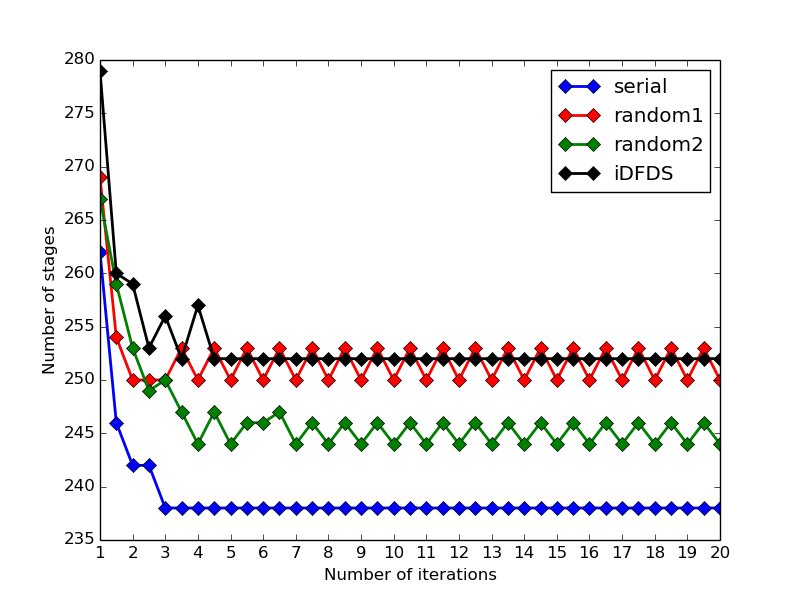
\includegraphics[width=7cm]{convergence_central_148}
    \caption{148 processors.}
  \label{convergence_central_148}
  \end{subfigure}
  \begin{subfigure}[b]{.5\textwidth}
    \centering
    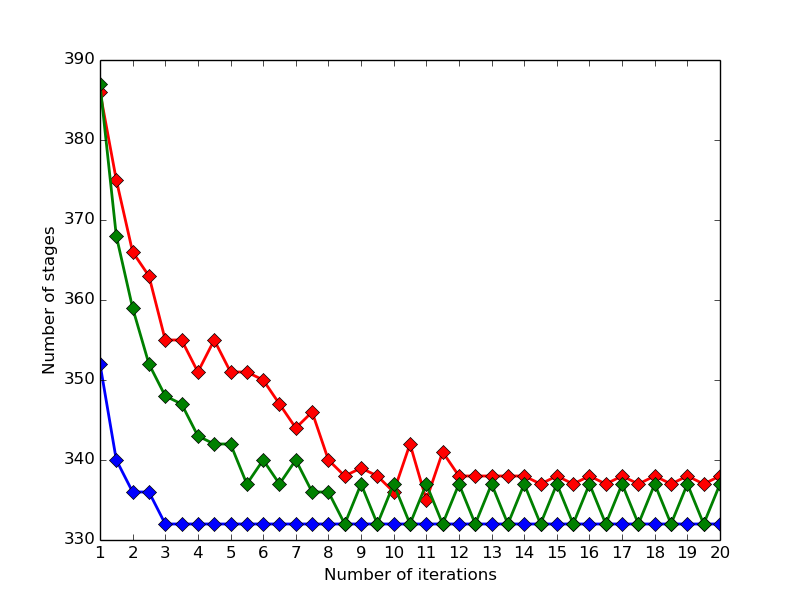
\includegraphics[width=7cm]{convergence_central_592}
    \caption{592 processors.}
  \label{convergence_central_592}
  \end{subfigure}
  \caption{Number of stages as a function of the number of CAP-PFB iterations.
  Half iterations correspond to backward iterations.}
\end{figure}

In the last case studied for this test, we do not allow for oscillations. If a
backward iteration, resp. forward iteration, produces a sweep worse than the
previous sweep, that sweep is disregarded and the best sweep is used in the
following forward iteration, resp. backward iteration. The results are shown in 
\Cref{amr_3}.
% Order of results: no seed, seed = 0, seed = 1.
% Table for new_amr_1 and new_amr_3 = refined mesh in the middle have been gather
\begin{table}[H]
  \begin{center}
    \begin{tabular}{|c|c|c|c|}
      \hline
      N.procs & Init. n. stages & Final n. stages & Iter. \\
      \hline
      148 & 2760 & 238 & 3 \\
      148 & 804  & 250 & 2 \\
      148 & 788  & 244 & 5 \\
      592 & 5520 & 332 & 3 \\
      592 & 1402 & 351 & 3 \\
      592 & 1364 & 337 & 6 \\
      \hline
    \end{tabular}
    \caption{Number of stages required to sweep through a mesh refined in the
      middle of the domain after gathering of the tasks without oscillations
    allowed.}
    \label{amr_3}
  \end{center}
\end{table}
There are three cases where the best scheduling is obtained after a
non-monotonic decrease, in one of them the best scheduling is obtained with the
new method. In the other two cases, the solution is the best scheduling obtained
in during the monotone phase.


\subsection{Second AMR test}
In this test, the mesh is given by \Cref{mesh_2}. Once the gathering of tasks is
done, each processor owns tasks that require one unit of work and tasks that
require four units of work.
\begin{figure}[H]
  \centering
  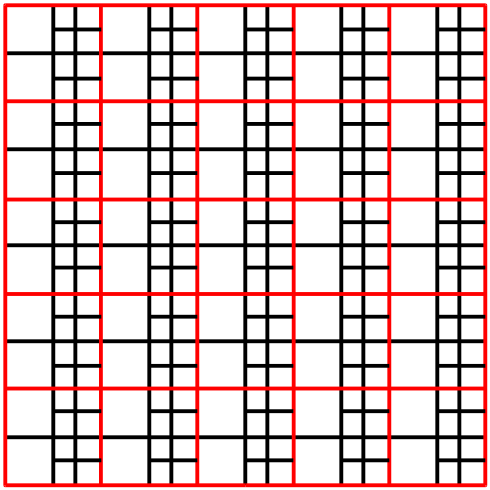
\includegraphics[width=5cm]{mesh_2}
  \caption{Mesh refined in the middle of the domain.}
  \label{mesh_2}
\end{figure}

First, we test the case where each processor owns 400 tasks (\Cref{band_1}).
\begin{table}[H]
  \begin{center}
    \begin{tabular}{|c|c|c|c|}
      \hline
      N.procs & Init. n. stages & Final n. stages & Iter. \\
      \hline
      $10 \times 10$ & 16808 & 518 & 3 \\
      $10 \times 10$ &  1841 & 562 & 6 \\
      $10 \times 10$ &  1832 & 541 & 6 \\
      $20 \times 20$ & 65618 & 882 & 2 \\
      $20 \times 20$ &  3488 & 882 & 3 \\
      $20 \times 20$ &  3435 & 882 & 5 \\
      \hline
    \end{tabular}
    \caption{Number of stages required to sweep through an adapted mesh.}
    \label{band_1}
  \end{center}
\end{table}

When using 100 processors, the results are very similar to what we had before.
However, when using 400 processors, all the final scheduling 
require the same number of stages. In \Cref{band_2}, we show the results when
each processor owns 160 tasks.

\begin{table}[H]
  \begin{center}
    \begin{tabular}{|c|c|c|c|}
      \hline
      N.procs & Init. n. stages & Final n. stages & Iter. \\
      \hline
      $10 \times 10$ & 3820 & 522 & 11 \\
      $10 \times 10$ & 1833 & 539 & 16 \\
      $10 \times 10$ & 1736 & 536 & 20 \\
      $20 \times 20$ & 9620 & 884 & 2  \\
      $20 \times 20$ & 3108 & 922 & 10 \\
      $20 \times 20$ & 3117 & 905 & 6  \\
      \hline
    \end{tabular}
    \caption{Number of stages required to sweep through an adapted mesh after
    gathering of the tasks.}
    \label{band_2}
  \end{center}
\end{table}

It is interesting to note that the final number of stages when using 400
processors is different for each initial scheduling. In \Cref{convergence_band},
we show the convergence of CAP-PFB. 

\begin{figure}[H]
  \begin{subfigure}[b]{.5\textwidth}
    \centering
    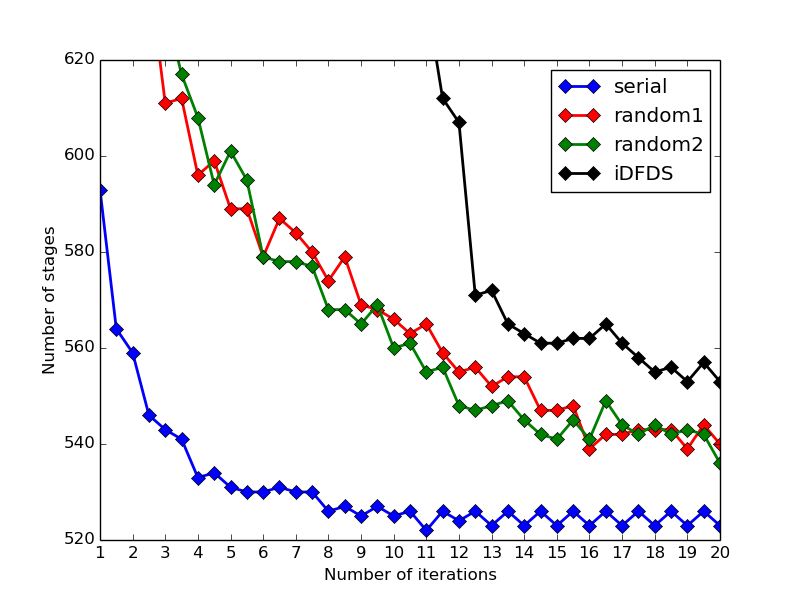
\includegraphics[width=7cm]{convergence_band_20_20}
    \caption{$10\times 10$ processors.}
  \end{subfigure}
  \begin{subfigure}[b]{.5\textwidth}
    \centering
    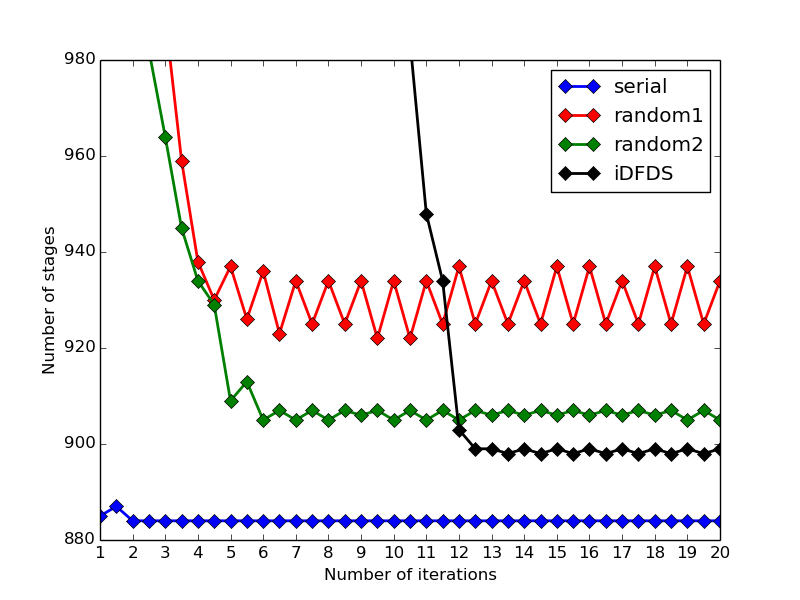
\includegraphics[width=7cm]{convergence_band_40_40}
    \caption{$20\times 20$ processors.}
  \end{subfigure}
  \caption{Number of stages as a function of the number of CAP-PFB iterations.
  Half iterations correspond backward iterations.}
  \label{convergence_band}
\end{figure}
 
We can see that the convergence is smoother and much faster when using more
processors which is the opposite of what we had in the previous test. In
\Cref{band_3}, we show the results when oscillations are not allowed.

\begin{table}[H]
  \begin{center}
    \begin{tabular}{|c|c|c|c|}
      \hline
      N.procs & Init. n. stages & Final n. stages & Iter. \\
      \hline
      $10 \times 10$ & 3820 & 533 & 4 \\
      $10 \times 10$ & 1833 & 580 & 5 \\
      $10 \times 10$ & 1736 & 594 & 5 \\
      $20 \times 20$ & 9620 & 884 & 3 \\
      $20 \times 20$ & 3108 & 923 & 8 \\
      $20 \times 20$ & 3117 & 907 & 7 \\
      \hline
    \end{tabular}
    \caption{Number of stages required to sweep through an adapted mesh after
    gathering of the tasks without oscillations allowed.}
    \label{band_3}
  \end{center}
\end{table}

We can see that using the proposed method, we get slightly better results than a
method which would stop as soon as scheduling is not better than the one obtain
at the previous iteration.

\section{Conclusions} \label{conclusions}
We have shown some preliminary results on the scheduling produced by CAP-PFB
when applied on uniform and AMR meshes. On uniform meshes, CAP-PFB was shown to
find an optimal scheduling. On AMR meshes, successive scheduling produced by
CAP-PFB do not lead monotonically to better scheduling. A simple method to
suppress the oscillations has been proposed and the importance of the initial
sweeping order was highlighted. Using a good initial sweeping order not only
produces a better final sweeping order but the convergence is smoothed. Future
works, include using CAP-PFB for real 2D and 3D applications and to study
different initial sweep ordering.


\bibliographystyle{unsrt}
\bibliography{database}

\end{document}

